\newpage

\section{Detailed description of $PTA\_PSP$ model}
\label{AnnexeModeles}
In this annex, we proposed a detailed description of each automaton that is part of the model $PTA\_PSP$. Let us recall that $PTA\_PSP$ model is composed of 7 Priced Timed Automata:
\begin{itemize}
	\item \texttt{Row start automaton (SA)}: manages the starting of spray in the row,
	\item \texttt{Movement automaton (MA)}: manages the movements of the sprayer inside the row from block to block,
	\item \texttt{Anticipation automaton (AA)}: selects the spraying command for the next vegetation block,
	\item \texttt{Control nozzles automaton (CA)}: manages the opening and closing of each nozzle according to the chosen spraying command,
	\item \texttt{Nozzles automata (NA$_i$)}: represent the behaviour of each nozzle (3 nozzles represented by 3 automata).
\end{itemize}

\subsection{\textbf{Row start automaton (SA)}}
This automaton, represented in the figure \ref{fig:start}, manages the startup phase. It sends a command event $"start0"$ to the \textit{anticipation automaton} to select a command for the first block. When selection is finished, it receives from the \textit{anticipation automaton}, a $"finishAnticipation"$ event. Then, it sends $"start1"$ event to the \textit{nozzle control automaton} to activate the nozzles for the first block. It waits $max\_temp\_open\_Nozzle$ the time required for nozzles to be opened. It sends to the \textit{movement automaton} a $"new \_block" $ event to start spraying at the first block. When spraying is finished it receives an $"endRow"$ event. When all nozzles are closed ($allClose == true$), it passes to the state $end$.

\begin{figure} [h!]
	\begin{center}
		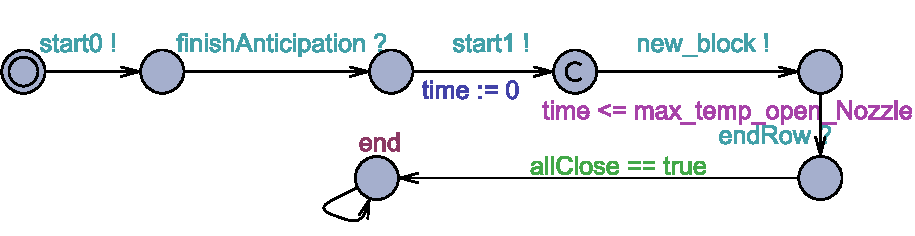
\includegraphics[width = 8cm]{Vegetation.pdf}
		\caption{Row Start automaton} \label{fig:start}
	\end{center}
\end{figure}


\subsection{\textbf{Anticipation automaton.}} This automaton, represented in the figure \ref{fig:ant}, makes it possible to select a command for the following block. The two possible commands for each vegetation block are $ C_ {best} $ and $ C_ {alt} $ which are stored respectively in $ CBest $ and $ CAlt $. \textit{The anticipation automaton} first receives the signal $"start0"$ from \textit{the Row Start automaton}. Then, if the value of the variable $ Choice $ is -1 (choice not predefined) then it chooses an order from $ CBest $ and $ CAlt $, stores its choice in the variable $ Choice $ and calls the function $ updateNextNozzle $. If $ Choice $ is predefined, then this choice is followed. Finally, \textit{the anticipation automaton} sends, in broadcast, the event $"finishAnticipation"$ and updates the variable $anticipe$ to \texttt{false} so as not to loop indefinitely.


\begin{figure}[h!]
	\begin{center}
		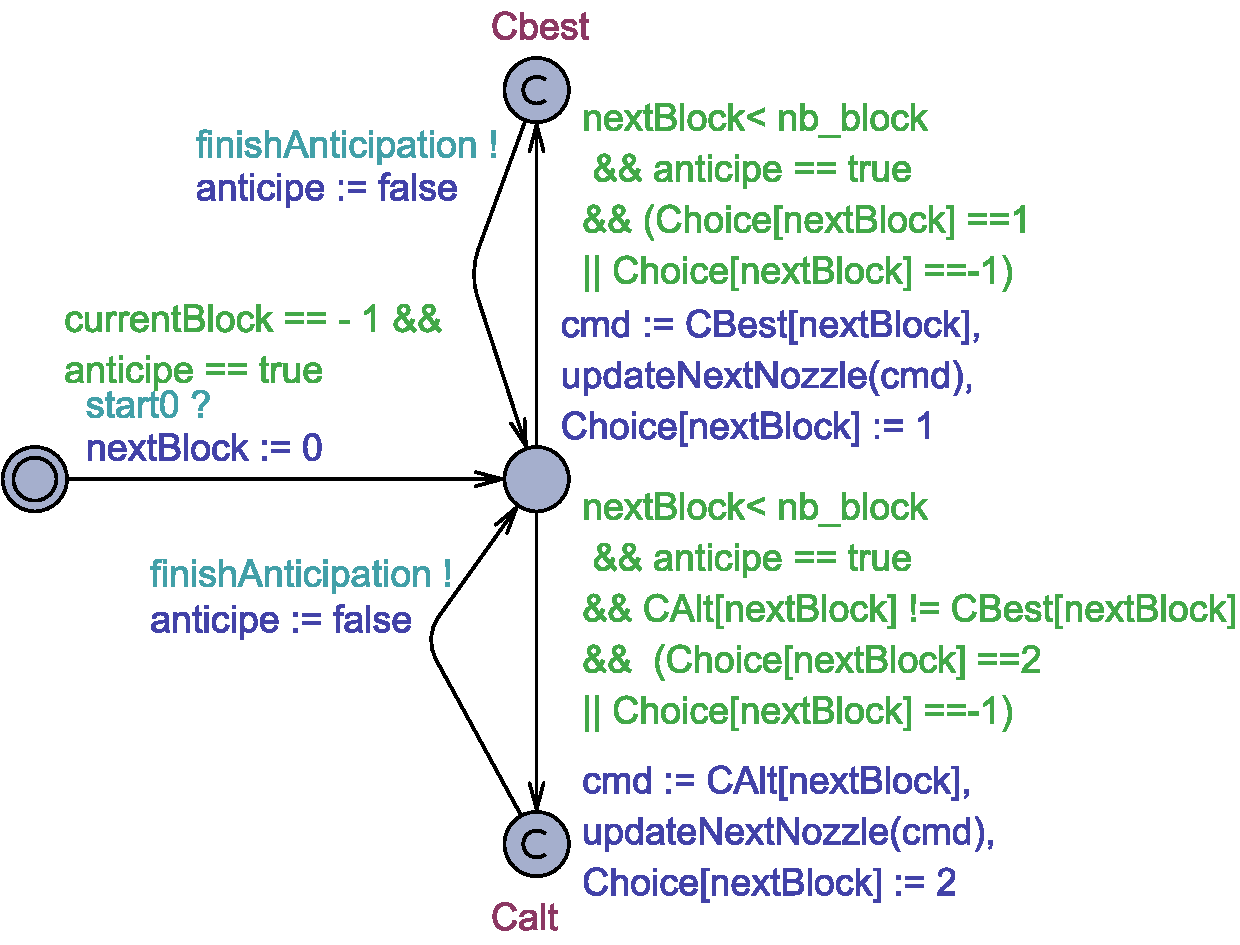
\includegraphics[width=9cm]{Anticipation.pdf}
		\caption{Anticipation automaton} 
		\label{fig:ant}
	\end{center}
\end{figure}

\subsection{\textbf{Movement automaton.}} This automaton, represented on the figure ~\ref{fig:dep}, allows to represent the movement of the sprayer. The time required to spray a vegetation block is computed in step 2, based on the length of the block and the speed of the sprayer. This information is stored in the $ tempo\_block $ variable. At the start,the sprayer is in the $"Init"$ state. When it receives the start event $"new\_block"$, it goes to the state $ block $. The state $ block $ has an invariant $ t\_block <= tempo\_block [currentBlock] $, the sprayer remain in this state for the duration of this block. The state $ block $ has also a guard $ t\_block == tempo\_block [currentBlock ] $ on its outgoing transitions, the automaton signals the end of a block by sending in broadcast the event $"new\_block"$ and the end of a row by sending in broadcast the event $"endRow"$ (it then returns to the state $ Init $).
\begin{figure}[h!]
	\begin{center}
		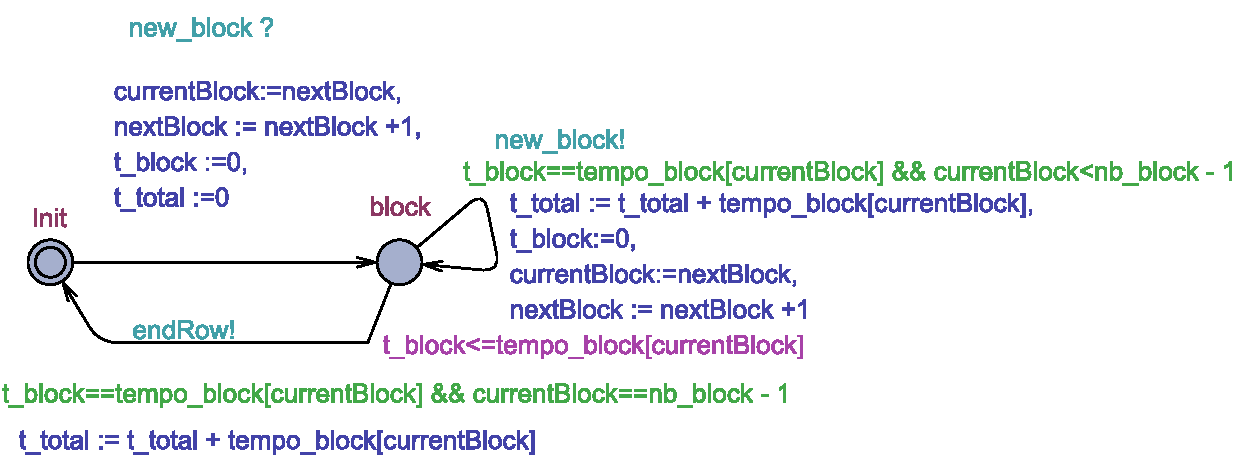
\includegraphics[scale=0.6, angle =90 ]{dep.pdf}
		\caption{Movement automaton} 
		\label{fig:dep}
	\end{center}
\end{figure}

\subsection{\textbf{Nozzles automata.}} These automata represent the behavior of each nozzle (figure \ref{fig:nozzle}). Each of these automata has four states: $OFF$ (initial state), $ON$, $TransitionOfOpen$ (opening) and $TransitionOfClose$ (closing). It receives the signals $"onNozzle"$ and $"offNozzle"$ to pass from a state to another. 
The nozzles response time, for opening or closing, is supposed to be a fixed and known ($ max \_temp\_open\_Nozzle $, $ max\_temp\_close\_Nozzle $). It is set at 0.2s in our example.

\begin{figure}[ht!]
	\begin{center}
		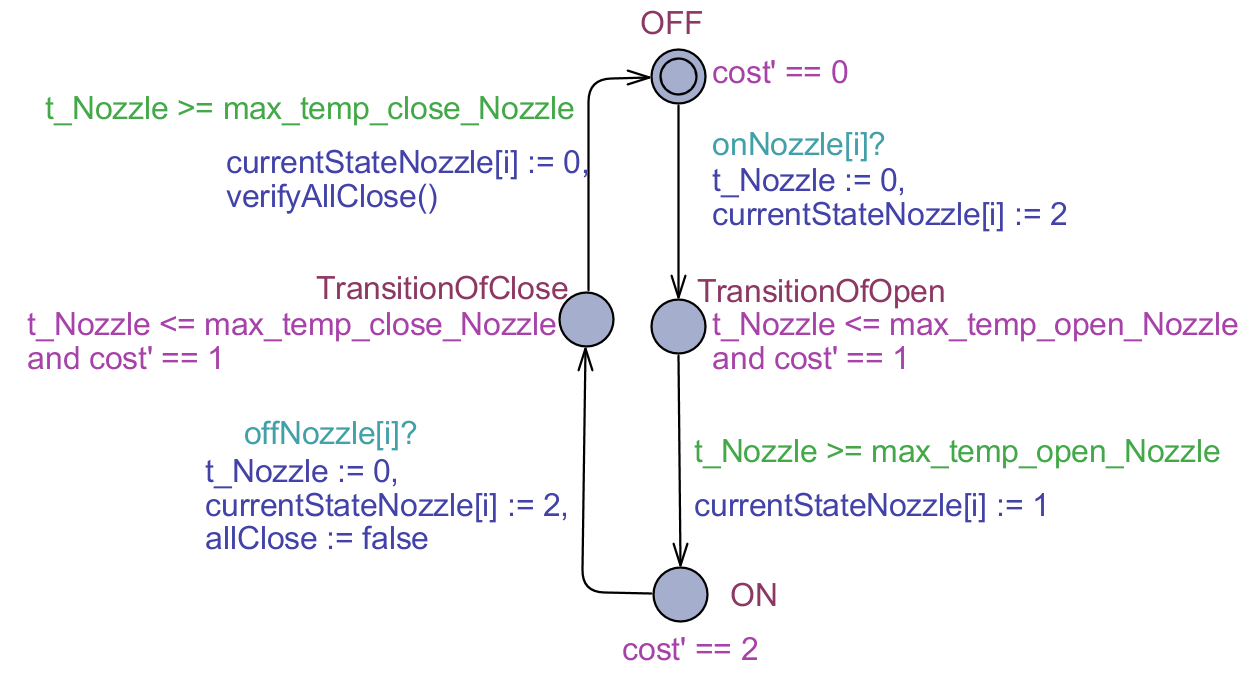
\includegraphics[scale = 0.8, angle =90]{nozzle.png}
		\caption{Nozzles automata} 
		\label{fig:nozzle}
	\end{center}
\end{figure}

\subsection{\textbf{Control Nozzles automaton.}} The role of this automaton, described in figure \ref{fig:CtrNozzle}, is to control the nozzles. When it receives the signal $ "finishAnticipation"$ from \textit{the Anticipation automaton}, it calls the function $control ()$ which determines the nozzles to be opened or closed for the next block. To secure the quantity of sprayed product in each block, the nozzles selected for opening are opened 0.2s before the start of the block (the value 0.2 is stored in the constant $ max\_temp\_open\_Nozzle $). Conversely, those which must be closed will not be completely closed until 0.2s after the block change (the value 0.2 is stored in the constant $ max\_temp\_close\_Nozzle $). To open a nozzle i, the \textit{nozzle control automaton} sends, 
$max\_temp\_open\_Nozzle $ before the end of the current block, the event $onNozzle [i]$  (see guard $t\_block <= tempo\_block[currentBlock]\-\ max\_temp\_open\_Nozzle $), and to close the nozzle i, it sends the event $offNozzle [i]$, after having received the synchronization event $new\_block$ from \textit{the movement automaton}. As soon as the commands on the nozzles are effective, then the variable $anticipe$ is set to $ True $ to allow anticipation for the next block.


\begin{figure}[h!] 
	\begin{center}
		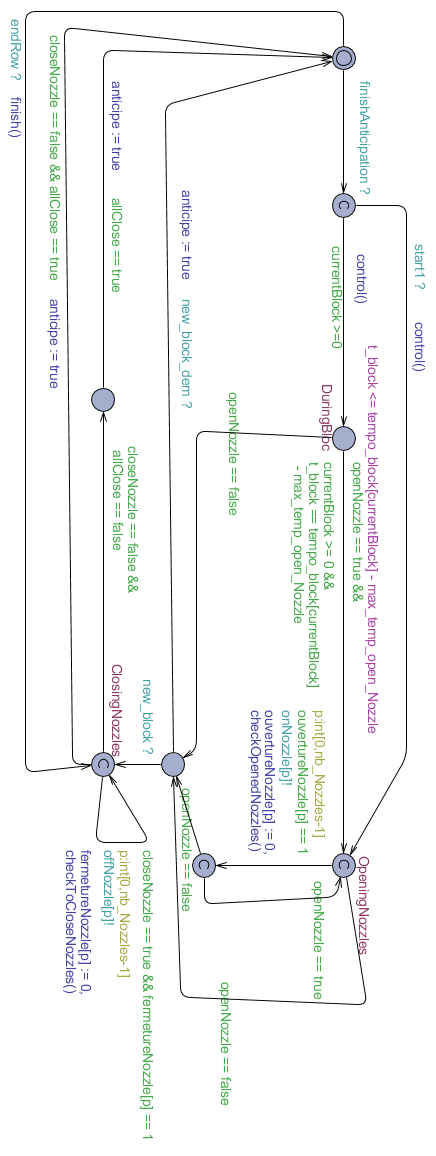
\includegraphics[scale = 0.7]{ControlBuse.png}
		\caption{Control Nozzles automaton} 
		\label{fig:CtrNozzle}
	\end{center}
\end{figure}
